%!TEX root = ../dissertation.tex
\begin{savequote}[125mm]
    The speaker wants to be understood. %, so he intends to speak in such a way that he will be interpreted in a certain way. 
    In order to judge how he will be interpreted, he uses his [...] starting theory of interpretation. % interpreter’s readiness to interpret along certain lines. %Central to this picture is what the speaker believes is 
%The speaker does not necessarily speak in such a way as to prompt the interpreter to apply this prior theory; he may deliberately dispose the interpreter to modify his prior theory. But the speaker’s view of the interpreter’s prior theory is not irrelevant to what he says, nor to what he means by his words; it is an important part of what he has to go on if he wants to be understood.
As speaker and interpreter talk, their ``prior'' theories become more alike; so do their ``passing'' theories. %The asymptote of agreement and understanding is when passing theories coincide. 
%But the passing theory cannot in general correspond to an interpreter’s linguistic competence. 
Not only does it have its changing list of proper names and gerrymandered vocabulary, but it includes every successful use of any other word or phrase, no matter how far out of the ordinary. 
Every deviation from ordinary usage, as long as it is agreed on for the moment (knowingly deviant, or not, on one, or both, sides), is in the passing theory as a feature of what the words mean on that occasion. 
Such meanings, transient though they may be, are literal.
\qauthor{\vspace{-2em}Donald Davidson, 1986}
\end{savequote}

\chapter{An inferential model of convention-formation}
\graphicspath{{./figures/modeling/}}

In this chapter, we present a computational model formalizing an account of how speakers coordinate on meaning under uncertainty. 
Our formal approach is grounded in the family of Rational Speech Act (RSA) models, which have been successful in explaining a wide range of linguistic phenomena---including scalar implicature \cite{GoodmanStuhlmuller13_KnowledgeImplicature}, adjectival vagueness \cite{LassiterGoodman15_AdjectivalVagueness}, overinformativeness \cite{degen2019redundancy}, indirect questions \cite{hawkins_why_2015}, and other non-literal language use \cite{KaoWuBergenGoodman14_NonliteralNumberWords}---as arising from a process of recursive social reasoning.% \cite{GoodmanFrank16_RSATiCS}. 
%Most previous applications of RSA have focused on the listener's problem of language comprehension, but the puzzle of conventionalization is primarily a puzzle of speaker production. 

At the core of any model of referential communication is the notion of a \emph{semantics} giving the meanings of utterances in the language. 
For the minimal examples in this chapter, it suffices to define a lexical function $\mathcal{L}: (w, o) \rightarrow \mathbb{R}$, assigning any word-object pair a real-valued meaning according to how well the word $w$ applies to the object $o$. 
This is a continuous generalization of classic truth-conditional semantics \shortcite{GrafEtAl16_BasicLevel}, where utterances may apply more or less well to different referents. 
For instance, the utterance \emph{dancer} may initially be expected to apply to a photorealistic image of a \texttt{ballerina} ($\mathcal{L}(\textit{dancer}, \texttt{ballerina}) = 0.99$) more than an abstract sketch of one ($\mathcal{L}(\textit{dancer}, \texttt{ballerina drawing}) =0.6$), but apply to both better than a non-category member like an image of dog falling down the stairs ($\mathcal{L}(\textit{dancer}, \texttt{dog}) = 0.05$).

In this framework, an $n$th order pragmatic speaker trying to refer to particular object $o \in \mathcal{O}$ assuming lexicon $\mathcal{L}$ selects an utterance $u \in \mathcal{U}$ by trading off its expected informativity (with respect to a rational listener agent) against its cost, usually based on length:
$$S_n(u | o, \mathcal{L}) \propto \exp{\left(\alpha \log L_{n-1}(o | u, \mathcal{L}) - \textrm{cost}(u)\right)}$$
where $\alpha$ is a soft-max optimality parameter controlling the extent to which the speaker maximizes over listener informativity. 
The listener, in turn, inverts the speaker model to reason about what underlying object $o$ the speaker is trying to convey, given their utterance $u$:
$$L_n(o | u, \mathcal{L}) \propto S_{n}(u | o, \mathcal{L})P(o)$$
\indent This recursion eventually bottoms out in a \emph{literal listener} who directly looks up the meaning of the utterance in the lexicon:
$$L_0(o | u, \mathcal{L}) \propto \mathcal{L}(u, o)\cdot P(o)$$

\section{Adapting to a single partner}
Now, we extend the lexicon from a lookup table or a static logical form into a dynamic, parameterized representation that can be constantly being updated.
To formalize this notion of semantic meaning, we begin with the additional assumption of \emph{lexical uncertainty} \cite{SmithGoodmanFrank13_RecursivePragmaticReasoningNIPS,BergenLevyGoodman16_LexicalUncertainty}. 
That is, instead of assuming agents have fixed knowledge of $\mathcal{L}$, we allow for uncertainty over the exact meanings of lexical items in the current context (e.g. it may be initially unclear what ``the dancer" might refer to). 
Concretely, we put a prior $P(\mathcal{L})$ over the identity of a partner's true lexicon, which may be initially biased toward certain meanings from previous experience. 

Bayesian updating then gives a rule for updating expectations about this true lexicon conditioned on repeated observations of a partner's behavior:
$$P_{L_n}(\mathcal{L} | d) \propto P(\mathcal{L})\prod_i S_n(o_i | u_i, \mathcal{L})$$
where $d = \{o_i, u_i\}$ is a set of observations containing utterances $u_i$ referring to objects $o_i$ from previous exchanges with that partner.
The listener marginalizes over this posterior when interpreting a new utterance $u$ from the speaker:
$$L_n(o | u, d) \propto \sum_\mathcal{L}P_{L_n}(\mathcal{L}|d)L_n(o | u,\mathcal{L})$$
The speaker, in turn, considers what utterances would be most informative for such a listener:
$$S_n(u | o, d) \propto \exp( \alpha\log\left(\sum_{\mathcal{L}} P_{S_n}(\mathcal{L} | d) L_{n-1}(o | u, \mathcal{L})\right) - \textrm{cost}(u) )$$
where the posterior over lexica $P_{S_n}(\mathcal{L} | d)$, uses the listener likelihood $L_{n-1}$ instead of the speaker likelihood:
$$P_{S_n}(\mathcal{L} | d) \propto P(\mathcal{L})\prod_i L_{n-1}(u_i | o_i, \mathcal{L})$$
For the purposes of this paper, we fix the depth of recursion at $n = 2$.
This model is implemented in the probabilistic programming language WebPPL \cite{GoodmanStuhlmuller14_DIPPL}. \footnote{These results can be reproduced running our code in the browser at \url{http://forestdb.org/models/conventions.html}}. 

\subsection{Model Results}

\begin{figure}
\centering
    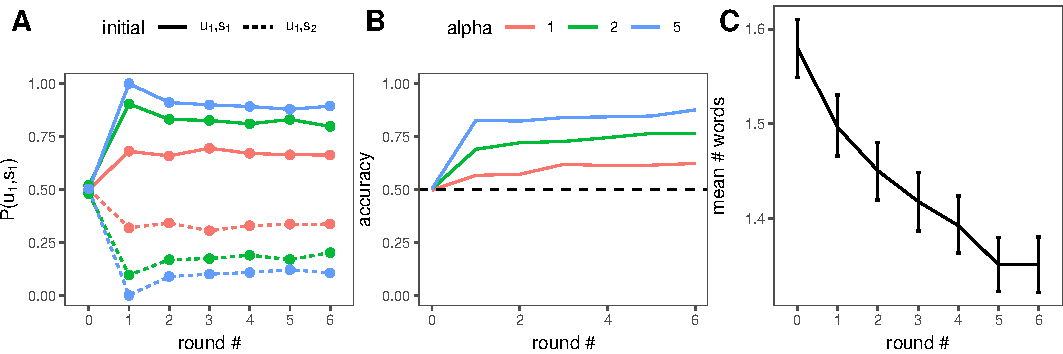
\includegraphics[scale=.8]{modelResults.pdf}
  \caption{Schematic of model}
  \label{fig:modelResults}
\end{figure}

\paragraph{Coordination}
First, we show how agents updating their meaning functions in this way can coordinate even in the absence of strong initial priors. 
The initial choices in an interaction can be taken as evidence for a particular lexicon and become the basis for successful communication, even when both speaker and listener are uncertain at the beginning.
As a simple test case, consider an environment with two objects ($\{o_1, o_2\}$), where the speaker must choose between two utterances ($\{u_1, u_2\}$) with equal production costs. 
For the prior $P(\mathcal{L})$ over the meaning of each utterance, we define a Beta distribution\footnote{In our implementation, we use exact enumeration over coarse-grained bins; experiments using variational inference on the full continuous distribution give similar results}, so on the first round both utterances are equally likely to apply to either shape. 
If the speaker were trying to get their partner to pick $o_1$, then because each utterance is equally (un)informative, they could only randomly sample one (say, $u_1$), and observe the listener's selection of a shape (say, $o_1$, a correct response). 
On the next round, the speaker uses the observed pair $\{u_1, o_1\}$ to update their beliefs about their partner's true lexicon, uses these beliefs to generate a new utterance, and so on. 
To examine expected dynamics over multiple rounds, we forward sample many possible trajectories.

We observe several important qualitative effects in our simulations. 
First, and more fundamentally, the evidence that a knowledgeable listener responded to utterance $u$ by choosing a particular object $o$ provides support for lexicons in which $u$ is a good fit for $o$. 
Hence, the likelihood of the speaker using $u$ to refer to $o$ will increase on subsequent rounds (see Fig.\ref{fig:modelResults}A). 
In other words, the initial symmetry between the meanings can be broken by initial random choices, leading to completely arbitrary but stable mappings in future rounds. 

Second, because the listener is updating their meaning representation from the same observations under the same set of assumptions, both partners converge on a \emph{shared} set of meanings; hence, the expected accuracy of selecting the target object rises on future rounds (see Fig. \ref{fig:modelResults}B). 
Third, because one's partner is assumed to be pragmatic via recursive Rational Speech Act mechanisms, agents can also learn about \emph{unheard} utterances. 
Observing $d = \{(u_1, o_1)\}$ also provides evidence that $u_2$ is \emph{not} a good fit for $o_1$.
This effect arises from Gricean maxims: if $u_2$ were a better fit for $o_1$, the speaker would have used it instead \cite{Grice75_LogicConversation}. 
Fourth, \emph{failed references} can lead to conventions just as effectively as successful references: if the speaker intends $o_1$ and says $u_1$, but then the listener incorrectly picks $o_2$, the speaker will take this as evidence that $u_1$ actually means $o_2$ in their partner's lexicon and become increasingly likely to use it that way on subsequent rounds.

\paragraph{Reduction}
Next, we show how our model explains reduction of utterance length over multiple interactions. 
For utterances to be reduced, of course, they must vary in length, so we extend our grammar to include \emph{conjunctions}. 
Conjunctions are one of the simplest ways to constructi longer utterances compositionally from lexical primitives, using the product rule:
$$\mathcal{L}(u_i \textrm{ and } u_j, o) = \mathcal{L}(u_i, o) \times \mathcal{L}(u_j, o)$$
\indent Analogous to the \emph{tangram} stimuli used in the reference game reviewed in Chapter 1, which have many ambiguous features and figurative perspectives that may be evoked in speaker descriptions, we consider a scenario the two objects $\{o_1, o_2\}$ differ along two different features. 
The speaker thus has four primitive words at their disposal -- two words for the first feature ($\{u_{11}, u_{12}\}$) and two for the second $\{u_{21}, u_{22}\}$. 
While we established in the previous section that conventions can emerge over a reference game in the complete absence of initial preferences, players often bring such preferences to the table. 
A player who hears `ice skater' on the first round of a tangrams task is more likely to select some objects more than others, even though they still have some uncertainty over its meaning in the context. 
To show that our model can accommodate this fact, we allow the speaker's initial prior meanings to be slightly biased. 
We assume $u_{11}$ and $u_{21}$ are a priori more likely to mean $o_1$ and $u_{12}$ and $u_{22}$ are more likely to mean $o_2$.

We ran 1000 forward samples of 6 rounds of speaker-listener interaction, and averaged over the utterance length at each round \footnote{In our simulations, we used $\alpha = 10$ and found the basic reduction effect over a range of different biases}. 
Our results are shown in Figure \ref{fig:modelResults}C: the expected utterance length decreases systematically over each round. 
To illustrate in more detail how this dynamic is driven by an initial rational preference for redundancy relaxing as reference becomes more reliable, we walk step-by-step through a single trajectory. 
Consider a speaker who wants to refer to object $o_1$. 
They believe their knowledgeable partner is slightly more likely to interpret their language using a lexicon in which $u_{11}$ and $u_{12}$ apply to this object, due to their initial bias. 
However, there is still a reasonable chance that one or the other alone actually refers more strongly to $o_2$ in the true lexicon. 
Thus, it is useful to produce the conjunction "$u_{11}$ and $u_{12}$" to hedge against this possibility, despite its higher cost. 
Upon observing the listener's response (say, $o_1$), the evidence is indeterminate about the separate meanings of $u_{11}$ and $u_{12}$ but both become increasingly likely to refer to $o_1$. 
In the trade-off between informativity and cost, the shorter utterances remain probable options. 
Once the speaker chooses one of them, the symmetry collapses and that utterance remains most probable in future rounds. 
In this way, meaningful sub-phrases are omitted over time as the speaker becomes more confident about the true lexicon. 

\section{Generalizing to new partners}

The model introduced in the previous section formally combines the first two mechanisms outlined in Chapter 1: a lexical prior and a learning mechanism to rapidly coordinate with a particular partner.
However, it leaves the question of \emph{generalization} unaddressed: what happens when we start talking to a new partner?
To what extent, if any, does an interaction with one partner change our expectations about the next? 
In this section, we propose a hierarchical generalization mechanism capturing how agents transfer what they have learned about one partner to another partner. 

This hierarchical structure --- sometimes termed a \emph{partial pooling} model --- can be understood in contrast to two simpler mechanisms, roughly corresponding to \emph{complete pooling} and \emph{no pooling} in multi-level statistical models \cite{gelman2006data}.
A complete pooling model simply ignores partner identity by updating a single internal model used with all partners. 
A no pooling model, on the other hand, maintains completely distinct partner-specific representations.
Like their statistical counterparts, these two theories of generalization in language face problems: each one is unable to explain the characteristic phenomena motivating the other. 
Ignoring partner identity will fail in the settings of interest in psycholinguistics where distinct information about one’s partner is available and relevant for conversation. 
On the other hand, entirely sealing off the meanings built up with one partner from expectations about others means speakers will revert to a fixed backdrop with each novel partner.

Hierarchical \emph{partial pooling} models offer a principled compromise between these extremes: agents equipped with such a model can integrate rich knowledge of specific partners with a mechanism for abstracting away what is common across different partners.
These models have been key to explaining how the human mind solves other difficult inductive problems in domains like causal learning \cite{KempGoodmanTenenbaum10_LearningToLearn,GoodmanUllmanTenenbaum11_TheoryOfCausality}, speech perception \cite{KleinschmidtJaeger15_RobustSpeechPerception} and concept learning \cite{KempPerforsTenenbaum07_HBM} where abstract, shared properties must be jointly inferred with idiosyncratic particulars of instances. 
Such a model has the potential to capture how agents make use of multiple levels of social structure across partners and communities. 

\begin{figure}
\centering
    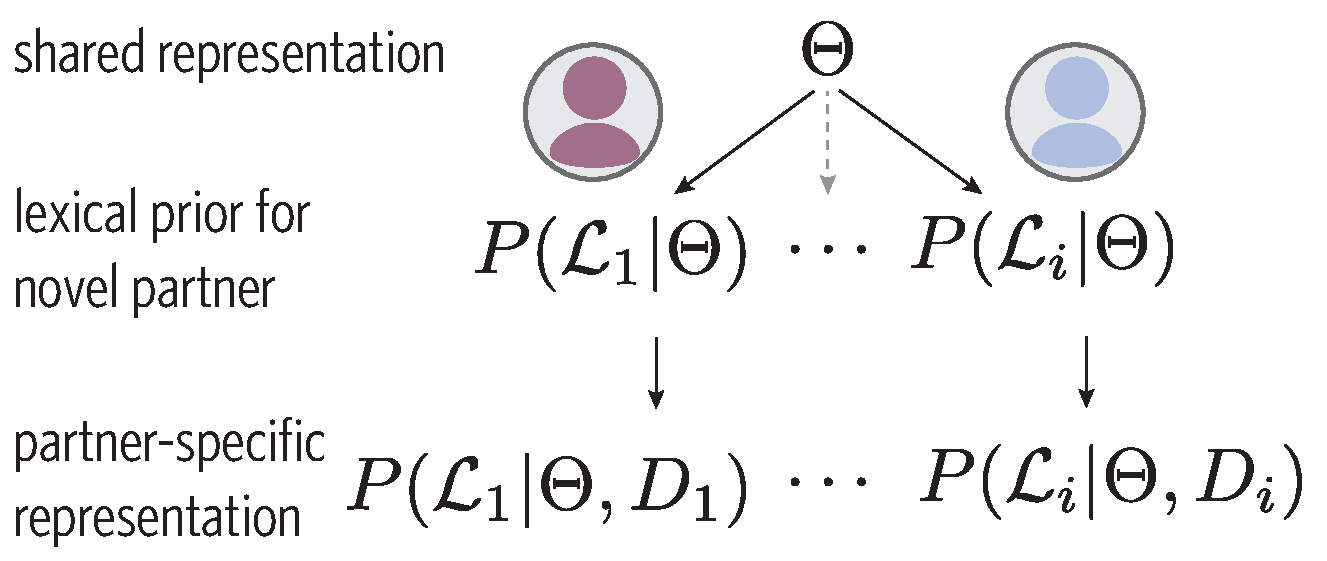
\includegraphics[scale=.45]{task1_model.pdf}
  \caption{Schematic of hierarchical model}
  \label{fig:task1model}
\end{figure}

We formalize this model as a straightforward extension of the RSA model above.
Specifically, we add an additional community-level representation parameterizing the lexical prior to create a hierarchical dependency structure (see Fig. \ref{fig:task1model}). 
%Here we sketch the ``ideal'' mathematical form of the proposed model, leaving implementational details for the following section.
At the highest level of the hierarchical lexical representation is a \emph{community-level} variable $\Theta$ parameterizing the agent's prior expectations for the likely lexicon $\mathcal{L}_i$ used by a novel community member $i$: $P(\mathcal{L}_i | \Theta)$. 
%For the conceptual purposes of this chapter, it is not important exactly what form this distribution takes, or what initial prior over the over-hypothesis $P(\Theta)$ could in principle guide early language learning
For simplicity, we generalize our Beta prior in the earlier section by assuming $\Theta$ is a tensor parameterizing a matrix containing an entry for every $(w,o)$ in the lexicon $\mathcal{L}_i$.  
We can then place an uninformative prior $P(\Theta)$ over that tensor which does not overwhelm the likelihood.
We will use a diagonalized multivariate Gaussian \cite<but see>[p. 110, for other reasonable choices]{gelman_bayesian_2014}. 
More generally, we could allow for arbitrarily complex dependencies between entries of the lexicon by using a neural network with weight tensor $\Theta$.
In Chapter 4, we will implement such a prior using an Empirical Bayes approach, only representing a point estimate of $\Theta$ rather than the whole distribution.
For now, it only matters that this knowledge is hierarchical: we expect all members of our language community to share some commonality in what they mean by things. 

Now that we have defined a hierarchical likelihood on lexical beliefs, we must say how we \emph{learn} partner-specific models. 
Our partner-specific beliefs about a particular individual's semantics $\mathcal{L}_i$ are formed by integrating our abstract lexical knowledge $\Theta$ with particular  observations $D_i$ of that particular individual, concretely, utterances and responses in a reference game:
$$%\begin{array}{rcl}
P(\mathcal{L}_i | D_i)  \propto \int_{\Theta}P(\mathcal{L}_i | D_i,  \Theta) P(\Theta | D_i) 
%                     & = & \mathbb{E}_{\Theta_0}[P(\mathcal{L}_i | \Theta_0, D_i)] 
%\end{array}
$$
where the posteriors in the integral can be computed using Bayes rule:
$$
P(\mathcal{L}_i | D_i, \Theta) \propto P(D_i | \mathcal{L}_i, \Theta) P(\mathcal{L}_i | \Theta)
$$
Note that our posterior beliefs about $\Theta$ are in fact informed by observations from \emph{all} speakers: $D = \bigcup_{i=1}^k D_i$. 
Additionally, because the partner-specific model depends on $\Theta$, Bayesian inference allows new data to systematically inform the shared, population-level representation as well (Fig. \ref{fig:task1model}).
Critically for predictions about generalization, new language data (i.e. particular ways of referring to the tangram shapes) may at first be more parsimoniously explained as an idiosyncratic property of a particular partner's lexicon, or ``idiolect''. 
If two or three partners all happen to use the same language, however, it starts to become more likely that a novel partner will share it as well (this transfer is sometimes referred to as ``sharing of statistical strength.'')
This formalizes the intuition sketched in Chapter 1.

%For  adult language users who have observed innumerable uses of language over their lifetimes, the contribution of a new data point to the overhypothesis $P(\Theta_0 | D)$ should be negligible; the contribution to a partner-specific model, however, can be quite strong. 

Finally, to fully specify our model and compute our partner-specific lexical posterior $P(\mathcal{L}_i | D_i, \Theta)$, we must link our beliefs about a partner's lexica to their actual behavior with a likelihood function $P(D_i | \mathcal{L}_i, \Theta)$. 
This is naturally supplied by the Rational Speech Act framework used in the previous section \cite{FrankGoodman12_PragmaticReasoningLanguageGames,GoodmanFrank16_RSATiCS,BergenLevyGoodman16_LexicalUncertainty,SmithGoodmanFrank13_RecursivePragmaticReasoningNIPS}: we assume speakers produce utterances that are parsimonious yet informative in context with respect to their lexicon, and listeners interpret utterances by inverting a speaker model. Because we expect our partner to use language rationally given some lexicon, the utterance they choose to refer to some object will be probable under some lexica and highly improbable under others. 
In this way, a particular agent's language use is a cue to their particular lexicon as well as a cue to the communal lexicon shared. 

In summary, our hierarchical model formalizes the intuition that global conventions are learned and generalized over repeated interactions with many different people, and that this shared semantic prototype is the backbone supporting rapid learning for new partners and situations. 

\paragraph{Model Results}

Our primary aim in this section is to examine the gradient of generalization produced by our hierarchical model across different partners.
To test this behavior, we used the same simple scenario with two objects and two words as we used to test adaptation to a single partner.
As our measure of interest, we focus on a listener agent's shifting expectations about which target is being referred to as they adapt their semantic representations.
Instead of presenting a stream of data from a single partner, however, we swap in a new partner every $k$ rounds of the reference game.

To derive quantitive behavior in this scenario, we must concretely specify the agent's lexical priors and a method to perform inference.
We used independent Gaussian distributions for each $\theta_{ij} \in \Theta$ as a hyper-prior and centered our partner-specific prior $\ell_{ij} \in \mathcal{L}$ at the shared value for a particular partner:
$$\begin{array}{rcl}
P(\theta_{ij}) & \sim & \mathcal{N}(0, 5)\\
P(\ell_{ij}) & \sim & \mathcal{N}(\theta_{ij}, 1)
\end{array}$$
The variances chosen in these priors are assumptions about how strongly adaptation is regularized. 
Using a higher variance for the hyper-prior than for the partner-specific prior corresponds to the assumption that the agent has substantial uncertainty over the population-level lexicon, but that individuals in the population shouldn't vary too much from whatever that lexicon is.

\begin{figure}
\centering
    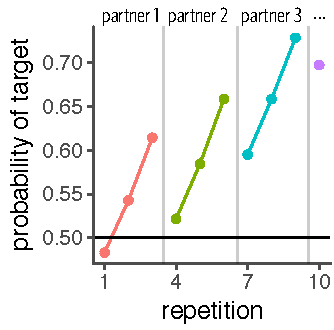
\includegraphics[scale=1.1]{partnerspecificity.pdf}
  \caption{Listener predictions as more evidence accumulated from different partners.}
  \label{fig:specificity}
\end{figure}

We used a variational method \cite<VI;>{RanganathGerrishBlei13_BlackBoxVariationalInference,blei_variational_2017} to perform inference in our model.
Variational methods transform probabilistic inference problems into optimization problems by approximating the true posterior with a parameterized family.
Specifically, we make a \emph{mean-field} approximation and assume that the full posterior can be factored into independent Gaussians for each random variable in the lexicon.
We then optimize the parameters of these posterior Gaussians by minimizing the evidence lower bound (ELBO) objective \cite<see>[for more details]{murphy2012machine}.
To examine how inferences change over time, we amortize inference. 
We run 10,000 steps of gradient descent on the first observation to obtain a lexical posterior, compute the listener's marginal prediction for the next observation, then continue running gradient descent on the same stored parameters after including the new observation in the data.

Our simulation results are shown in Fig. \ref{fig:specificity}.
To observe behavior in the simplest case, we feed the model the same object-target pair ($\{o_1, w_1\}$) on every trial.  
We find that the adapting listener begins at chance because of its uninformative prior, but after interacting with that partner for several rounds, it adapts its semantics to select the target well above chance. 
When a new partner is introduced, however, it reverts nearly to its original state: because of the hierarchical structure of its lexical expectations, it was ambiguous whether the evidence from the first partner was idiosyncratic or due to shared structure.
After adapting similarly to the second partner, however, it begins its interaction with a third partner with nearly the accuracy at the end of its interaction with the first partner.
Thus, expectations about an individual partners' semantics are gradually being incorporated into community-level expectations.

\section{Discussion}

This chapter advanced an \emph{inferential} theory of meaning in which agents continually adapt their beliefs about the semantics used by their partner.
We formalized this approach by integrating three core cognitive mechanisms in a probabilistic framework: (1) initial uncertainty about what a partner thinks words mean, (2) a mechanism for updating beliefs from observations of language use in context, and (3) a hierarchical structure for graded generalization to new partners.
Across several simulations, we showed that agents equipped with these mechanisms coordinate on increasingly accurate and efficient conventions with different partners.

This inferential model situates semantic meaning within a broader class of computational challenges facing agents in a constantly changing world.
Critically, the heavy lifting is done by domain-general learning mechanisms rather than specialized language modules: similar inferential mechanisms have been used to understand how internal representations are adapted for motor control \cite{berniker2008estimating}, speech perception \cite{KleinschmidtJaeger15_RobustSpeechPerception}, and visual perception \cite{austerweil2013nonparametric}.
What makes the problem of semantic adaptation distinctive, however, is its reliance on \emph{social inference}.
The relevant functional quantity for communicative understanding is the latent semantic representation used by another (rational) social agent in context. 
Instead of assuming that a single true semantics independently exists, agents assume each partner has their own idiosyncratic representations.
They must then infer the conventions at play using a generative model of their partner's behavior over the course of interaction.

This social component of our inferential approach contrasts in several ways with prior theories of adaptation in language use. 
First, we contrast the mechanisms in our model with the lower-level priming mechanisms proposed in the influential \emph{interactive alignment} account \cite{pickering2004toward, pickering2006alignment, garrod2009joint}.
According to this account, coordination on the higher-level mental representations necessary for successful communication proceeds primarily through automatic and egocentric imitation of surface statistics at lower levels. 
By appealing to classic spreading-activation connectionist models \cite<e.g.>{roelofs1992spreading}, \citeA{pickering2004toward} have argued that activating phonetic or syntactic features that are associated with specific lemmas in the lexicon can percolate to strengthen higher semantic levels of representation \cite{pickering1998representation}.
Thus, unconsciously coupling word choices \cite{louwerse2012behavior}, syntax \cite{gruberg2019syntactic,levelt1982surface}, body postures \cite{lakin2003using}, speech rate \cite{giles1991contexts}, or even informational complexity \cite{abney2014complexity} in dialogue can contribute to the coordination of higher-level semantic representations.

We fully expect that these low-level priming effects are at play in repeated reference tasks --- they are inescapable in any memory-based retrieval process.
But two signature phenomena are unable to be explained from priming mechanisms alone: \emph{partner-specificity} and \emph{reduction}.
If a particular semantic representation has been activated due to precedent in the preceding dialogue, then the identity of the speaker should not alter its continued influence \cite{brennan2009partner}.
Thus, egocentric priming-based theories are inconsistent with the empirical evidence of partner-specificity reviewed in Chapter 1.\footnote{Of course, more sophisticated memory retrieval accounts that represent different partners as different \emph{contexts} \cite<e.g>{polyn2009context} are consistent with partner-specificity. But evoking such an account presupposes that social information like partner identity is already a salient and relevant feature of the agent's context representation and thus no longer relies purely on ``egocentric'' activation mechanisms. In fact, socially-aware context reinstatement for episodic memory (with slower consolidation of ``shared'' conventions) would be a valid candidate for a process-level realization of our computational-level model.}
Furthermore, the gradual reduction of the speaker's utterance length is not obviously imitating any features of the listener's language use. 
Explaining why speakers think they can get away with shorter descriptions given sparse evidence of understanding (e.g. a correct response or a simple gesture of confirmation) and resort to longer descriptions given evidence of misunderstanding (e.g. an incorrect response) requires a mechanism for semantic coordination in the absence of lower-level statistics.

The phenomena of reduction and partner-specificity also pose challenges for computational models of convention formation that rely on simple variants of reinforcement learning \cite{steels_self-organizing_1995,barr_establishing_2004,young_evolution_2015,baronchelli_emergence_2018}.
While a variety of different models fall under this category, they all share some mechanism that makes utterances more likely to be produced after communicative successes and less likely after communicative failures.
Because agents in these models use a single (egocentric) representation of linguistic conventions irrespective of one's partner, they could not account for patterns of partner-specificity if these agents were placed in a series of repeated reference games. 
And again, it is not clear how naively reinforcing initially long descriptions could lead to reduction\footnote{It is plausible that using more sophisticated reinforcement schemes on neural architectures incorporating compositionality or recurrence into production \cite<e.g>{lazaridou2018emergence} could yield reduction with the addition of a cost term. Such a scheme would be similar in spirit to the adaptive neural agent we propose in Chapter 3.}.
Still, a clear success of these models is their focus on the conditions under which community-level convergence may be achieved, and it is imperative for future work to conduct similar large-scale simulations of an inferential model.

%A second theory is that speakers maintain separate representations of the meanings shared with each social partner. 
%In the simplest versions of this theory, information built up through the distinct history of interaction with one partner should crucially \emph{not} generalize to other partners \cite{clark_using_1996,brennan_partner-specific_2009,horton_revisiting_2016}.
%This idea has been fundamental for explaining the flexibility with which speakers adapt and switch between different social partners \cite{ClarkWilkesGibbs86_ReferringCollaborative,MetzingBrennan03_PartnerSpecificPacts} over the shorter timescales of language use studied in psycholinguistics.
%
%\todo[inline]{Also note that we're not exactly just implementing the full 'mutual knowledge' theory}
%These prior theories vary in the extent to which social reasoning about common ground is required. 
%Our agents lie on a spectrum spanning from the to the more sophisticated \emph{collaborative reference} theory of Clark \& Wilkes-Gibbs (1986).%, who collaboratively build up explicit representations of mutual knowledge. 
%They make critical use of pragmatic, social reasoning in order to learn meanings, but do not explicitly consider the fact that this history is shared, or represent their partner's own uncertainty.
%Speakers and listeners in our model implicitly coordinate their beliefs through a shared history of observations, which serves as a minimal form of ``common ground.''

Another key direction for future work is to account for richer forms of feedback.
Our simulations used the simplest source of feedback: the utterance and response in a reference game.
But listeners commonly respond using verbal back-channels (\emph{uh-huh}, \emph{hmmm}) or more sophisticated responses such as confirmation, suggestion, repair, or even follow-up questions. 
Without elaborating the generative model of the listener to include these verbal behaviors, we cannot explain the inferences a speaker will make upon hearing them.
Such an elaboration will thus be critical to explaining why listeners send fewer messages over time and what impact early listener responses on conventionalization. 

%These phenomena may also require our model to deal with planning over extended dialogues, and to potentially weaken the assumption that one's partner knows the true lexicon with complete certainty. 
%
%Similarly, while our model was explicitly designed with linguistic conventions in mind, it remains to be seen whether the same formulation generalizes to broader behavioral conventions. 
%For example, the real-time coordination games used in Hawkins \& Goldstone (2016) may not require players to reason about a structured lexicon with noise, but an action policy representation may play a similar role. 
%While there remain many complex aspects of convention-formation in communication games left for future research, our approach nonetheless serves as a lower bound on the degree of social reasoning needed to capture lexical conventions in these games.
